\documentclass[../main.tex]{subfiles}
\graphicspath{{\subfix{../Images/}}}
\begin{document}
\section{Equations \& Inequalities}

\subsection{Solving Equations using GC}
\subsubsection{Graphical Method}
Graph out the left and right side of the equation \\*
as 2 seperate graphs and solve for it's intercept

\subsubsection{Equation Solver (Not Recommended)}
Press the \textbf{math} button and select the Numeric Solver Option
and key in the LHS and RHS of the equation \\
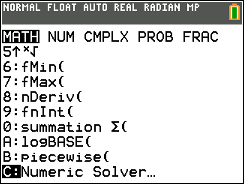
\includegraphics[scale=0.5]{B1 Equations & Inequalities/Capture 1.png}
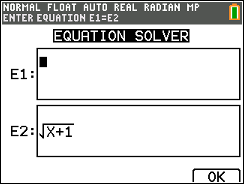
\includegraphics[scale=0.5]{B1 Equations & Inequalities/Capture 2.png} \\
Do note that you would have to key a guess (in this case it's \(x=0\))
before you are able to solve for the equation (by pressing \textbf{graph}) \\
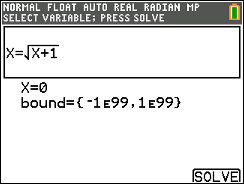
\includegraphics[scale=0.5]{B1 Equations & Inequalities/Capture 3.png}
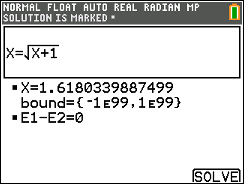
\includegraphics[scale=0.5]{B1 Equations & Inequalities/Capture 4.png}\


\subsection{System of Linear Equations}
An equation is linear when the variables have a power of 1 \\
\boxedeq{\text{General Form : } \sum_{i=1}^{n} \left(a_{i}x_{i}\right)=b \text{, where } a_{i},b \, \in \mathbb{R}}
\noindent
\begin{tabularx}{0.43\textwidth} {
    | >{\centering\arraybackslash}X
    | >{\centering\arraybackslash}X |}
    \hline
    Linear Equations & Non-Linear Equations \\
    \hline
    \(x-2y+3z=180\),  & \(xy=1\), \\
    \(2x_{1}+x_{2}-10x_=350\)  & \(x^{2}+3y=1\) \\
    \hline
\end{tabularx} \\\\
A System of Linear Equations have 3 possible outcomes
\begin{itemize}
    \item Exactly one Solution (Unique)
    \item Infinitely many Solutions
    \item No Solutions
\end{itemize}
No Solution \(\implies\) Inconsistent \\
At least 1 Solution \(\implies\) Consistent

\subsubsection{Solving with GC}
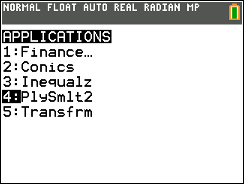
\includegraphics[scale=0.5]{B1 Equations & Inequalities/Capture 5.png}
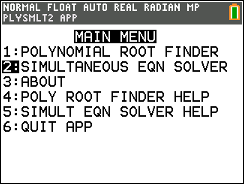
\includegraphics[scale=0.5]{B1 Equations & Inequalities/Capture 6.png} \\
We can use the simultatneous equation solver under the \\*
'pltSmlt2' App to solve our system \\
\underline{When a system has infinitely many solutions} \\
The solutions are represented with a 'free' variable \\
Example:
\begin{align*}
    x &= z - 2 \\
    y &= 3z + 2 \\
    z &= z
\end{align*}
In this case, \(z\) is the 'free' variable that determines the \\*
values of \(x\) \& \(y\), thus it has infinitely many solutions. \\*
The unique solution is determined by the context given \\\\
Example : If \(z=3\), then \(x=1\), \(y=11\)

\subsection{Inequalities}
\subsubsection{Basic Concepts}
Let \(a,b,c,d \in \mathbb{R}\) \\
\begin{tabularx}{0.43\textwidth} {
    | >{\centering\arraybackslash}X |}
    \hline
    \textbf{Properties} \\
    \hline
    If \(a>b\) \& \(b>c\), then \(a>c\) \\
    \hline
    If \(a>b\) \& \(c>0\), then \(ac>bc\) \& \(\displaystyle \left(\frac{a}{c}>\frac{b}{c}\right)\) \\
    \hline
    If \(a>b\) \& \(c<0\), then \(ac<bc\) \& \(\displaystyle \left(\frac{a}{c}<\frac{b}{c}\right)\) \\
    \hline
    If \(a>b\) \& \(c>d\), then \(a+c>b+d\) \\
    But \(a-c>b-d\) may not be true \\
    \hline
    If \(a>b>0\) \& \(n>0\), \\
    then \(a^n>b^n\) \& \(\displaystyle \left(\frac{1}{a^n}<\frac{1}{d^n}\right)\) \\
    \hline
    If \(a>b\),  \\
    then \(f(a)>f(b)\) if f is monotonic increasing \\
    then \(f(a)<f(b)\) if f is monotonic decreasing \\
    \hline
\end{tabularx}
\newpage \noindent

\subsubsection{Polynomial Inequalities}
For such inequalities in the form \(f(x) \geq 0\) or other \\*
inequality signs We can solve it by looking at the general  \\*
shape of the function or the test point method, after  \\*
determining the roots of the equation \\\\
\textbf{General shape of polynomials with even degrees} \\
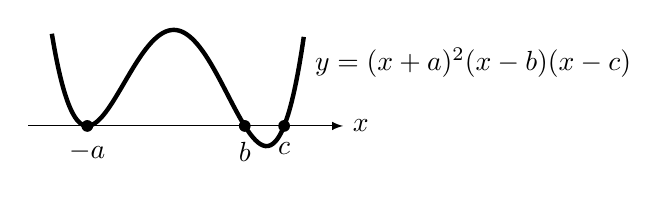
\begin{tikzpicture}[scale=0.5]
	% Draw x-axis
	\draw[-latex] (-4.5,0) -- (3.5,0) node[right] {\(x\)};

	% Draw function
	\draw[samples=100,domain=-3.9:2.5,smooth,variable=\x,black,ultra thick] plot ({\x},{0.1*(\x-1)*(\x+3)^2*(\x-2)}) node[below right] {\(y=(x+a)^2(x-b)(x-c)\)};

	% Label x-intercepts
	\node[circle,fill,inner sep=1.5pt,label={below:\(b\)}] at (1,0) {};
	\node[circle,fill,inner sep=1.5pt,label={below:\(-a\)}] at (-3,0) {};
	\node[circle,fill,inner sep=1.5pt,label={below:\(c\)}] at (2,0) {};
\end{tikzpicture} \\
\textbf{General shape of polynomials with odd degrees} \\
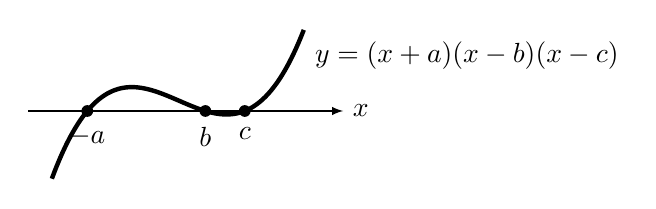
\begin{tikzpicture}[scale=0.5]
	% Draw x-axis
	\draw[-latex] (-4.5,0) -- (3.5,0) node[right] {\(x\)};

	% Draw function
	\draw[samples=100,domain=-3.9:2.5,smooth,variable=\x,black,ultra thick] plot ({\x},{0.1*(\x)*(\x+3)*(\x-1)}) node[below right] {\(y=(x+a)(x-b)(x-c)\)};

	% Label x-intercepts
	\node[circle,fill,inner sep=1.5pt,label={below:\(b\)}] at (0,0) {};
	\node[circle,fill,inner sep=1.5pt,label={below:\(-a\)}] at (-3,0) {};
	\node[circle,fill,inner sep=1.5pt,label={below:\(c\)}] at (1,0) {};
\end{tikzpicture} \\
\textbf{Steps to Solve the inequality}
\begin{enumerate}
    \item Make the term with the highest power is positive
    \item Factorize the equation
    \item Draw a number line with the roots of the equation
    \item By either graph or test point, determine the sign of each section\\* A section is the "gap" between roots and the ends
    \item Write out the final inequality
\end{enumerate}
Graph method is to mentally graph out the shape of the graph to
determine the sign of each section, while  test point is to test
a number within that section (e.g using \(1\) for \(0<x<2\)) to
determine the sign \\\\
Example : \((x-1)(x-2)(x-3)>0\) \\\\
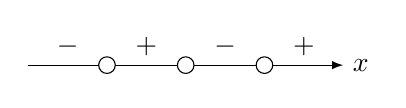
\begin{tikzpicture}
	% Draw number line
	\draw[-latex] (0,0) -- (4,0) node[right] {\(x\)};

	% Draw hollow circles at x=2 and 3
	\draw[fill=white] (1,0) circle (3pt);
	\draw[fill=white] (2,0) circle (3pt);
	\draw[fill=white] (3,0) circle (3pt);

    % Signs
	\draw[fill=black] (0.5,0) circle (0pt) node[above] {\(-\)};
	\draw[fill=black] (1.5,0) circle (0pt) node[above] {\(+\)};
	\draw[fill=black] (2.5,0) circle (0pt) node[above] {\(-\)};
	\draw[fill=black] (3.5,0) circle (0pt) node[above] {\(+\)};
\end{tikzpicture} \\
\(\therefore 1<x<2 \text{ or } x>3\) \\
\(\{x \in \mathbb{R} : 1<x<2 \text{ or } x>3\}\)
\newpage \noindent

\subsubsection{Inequalities involving Rational Functions}
Such inequalities can be solved with a similar method outlined in 2.3.2
\begin{enumerate}
    \item Express the inequality in the form such that one side is 0 \(\left(\text{e.g. }\displaystyle \frac{g(x)}{h(x)}>0\right)\)
    \item Make the term with the highest power is positive
    \item Factorize the polynomials
    \item By either graph or test point, determine the sign of each section\\* A section is the "gap" between roots and the ends
    \item \textbf{Check that the  x value(s) where the denominator = 0 isn't included}
\end{enumerate}
Example : \(\displaystyle \frac{(x-1)^{2}}{(x-3)} \geq 0\) \\\\
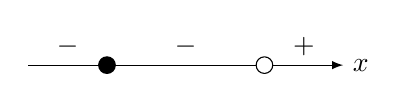
\begin{tikzpicture}
	% Draw number line
	\draw[-latex] (0,0) -- (4,0) node[right] {\(x\)};

	% Draw hollow circles at x=2 and 3
	\draw[fill=black] (1,0) circle (3pt);
	\draw[fill=white] (3,0) circle (3pt);

    % Signs
	\draw[fill=black] (0.5,0) circle (0pt) node[above] {\(-\)};
	\draw[fill=black] (2,0) circle (0pt) node[above] {\(-\)};
	\draw[fill=black] (3.5,0) circle (0pt) node[above] {\(+\)};
\end{tikzpicture} \\
\(\therefore x>3 \text{ or } x=1\) \\
\(\{x \in \mathbb{R} : x>3 \text{ or } x=1\}\)

\subsubsection{Inequalities involving Modulus Functions}
Let \(x,y \in \mathbb{R}\) and \(a>0\) \\
\begin{tabularx}{0.43\textwidth} {
    | >{\centering\arraybackslash}X |}
    \hline
    \textbf{Properties} \\
    \hline
    \(|x|>a \iff x<-a \text{ or } x>a\) \\
    \(|x|<a \iff -a<x<a\) \\
    \hline
    \(|x|<|y| \iff x^{2}<y^{2}\) \\
    \(|x|>|y| \iff x^{2}>y^{2}\) \\
    \hline
    \(|x^{2}|=|x|^{2}=x^{2}\) \\
    \(|xy|=|x||y|\) \\
    \(\sqrt{x^{2}}=|x|\) \\
    \hline
    \(|x-y|=|y-x|\) \\
    \hline
    \(\displaystyle \left|\frac{x}{y}\right| = \frac{|x|}{|y|}\) \\
    \hline
\end{tabularx} \\\\
Modulus Inequalities can be solved using these properties by
maniplulating the inequality or by a graphical method (2.3.5)
\newpage \noindent

\subsubsection{Using a Graphical Method}
Sketching the LHS and RHS of an inequality to determine the range of values \\\\
Example : \(|x|-|0.5x+1|>1\) \\
We can sketch the graphs \(y=|x|\) \& \(y=1+|0.5x+1|\) \\\\
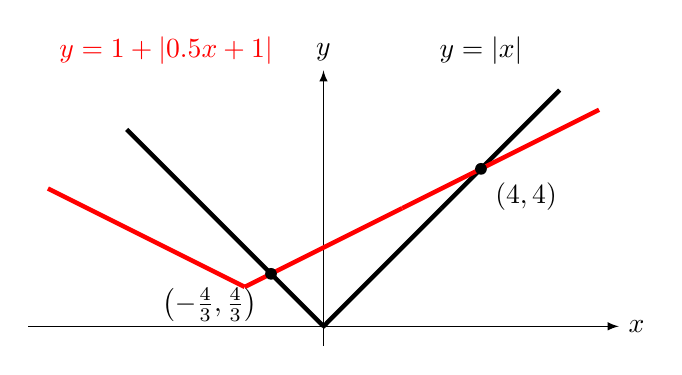
\begin{tikzpicture}[scale=0.5]
	% Draw axes
	\draw[-latex] (-7.5,0) -- (7.5,0) node[right] {\(x\)};
	\draw[-latex] (0,-0.5) -- (0,6.5) node[above] {\(y\)};

	% Draw y=|2x-1|
	\draw[samples=100,domain=-5:3,smooth,variable=\x,black,ultra thick] plot ({\x},{abs(\x)});
	\draw[samples=100,domain=3:6,smooth,variable=\x,black,ultra thick] plot ({\x},{abs(\x)});

	% Draw y=2+|x+1|
	\draw[samples=100,domain=-7:-2,smooth,variable=\x,red,ultra thick] plot ({\x},{1+abs(0.5*\x+1)});
	\draw[samples=100,domain=-2:2,smooth,variable=\x,red,ultra thick] plot ({\x},{1+abs(0.5*\x+1)});
	\draw[samples=100,domain=2:7,smooth,variable=\x,red,ultra thick] plot ({\x},{1+abs(0.5*\x+1)});

	% Label graphs
	\node[black] at (4,7) {\(y=|x|\)};
	\node[red] at (-4,7) {\(y=1+|0.5x+1|\)};

    % Labelling Coordinates of intercepts
	\node[circle,fill,inner sep=1.5pt,label={below left:\(\left(-\frac{4}{3},\frac{4}{3}\right)\)}] at (-4/3,4/3) {};
	\node[circle,fill,inner sep=1.5pt,label={below right:\((4,4)\)}] at (4,4) {};
\end{tikzpicture} \\
We would have to solve for the points of intercepts algebratically
and by referring to our graph, we can determine the solution set to the inequality,
which in this case is \(\displaystyle x<-\frac{4}{3} \text{ or } x>4\)

\subsubsection{Using Substitution}
This method is usually used when solving for an inequality with
a similar form to one that was solved in a previous part of a question \\\\
Example : Solve the inequality \(\displaystyle \frac{4-x}{x-2}>3\), \\* hence solve \(\displaystyle \frac{6x-2}{1-2x}>2\) \\\\
Manipulate \(\displaystyle \frac{6x-2}{1-2x}>2\) to a similar form of \(\displaystyle \frac{4-x}{x-2}>3\)
\begin{align*}
    \displaystyle \frac{6x-2}{1-2x}>2 \\
    \displaystyle \frac{6x-2}{1-2x}+1>3 \\
    \displaystyle \frac{6x-2+1-2x}{1-2x}>3 \\
    \displaystyle \frac{4x-1}{1-2x}>3 \\
    \displaystyle \frac{\frac{1}{x}}{\frac{1}{x}}\left(\frac{4x-1}{1-2x}\right)>3, \; x \neq 0 \\
    \displaystyle \frac{4-\frac{1}{x}}{\frac{1}{x}-2}>3
\end{align*}
Thus we had arrived at a similar form, and we can use
the substitution \(u=\frac{1}{x}\) to solve the inequality. \\
Note that now other than \(\displaystyle x \neq \frac{1}{2}\), \(x \neq 0\) too

\end{document}